\documentclass[11pt]{article}
\usepackage[a4paper,margin=1in]{geometry}
\usepackage{amsmath,amssymb,amsthm}
\usepackage{graphicx,float,microtype,booktabs,array}
\usepackage{xcolor}
\usepackage[colorlinks=true,linkcolor=blue!55!black,urlcolor=blue!60!black]{hyperref}
\newcommand{\R}{\mathbb R}
\newcommand{\Htilde}{\widetilde H}
\newcommand{\Wtilde}{\widetilde W}
\title{Two Questions from Fractional Adams--Moser--Trudinger Inequalities\\Were Answered by Hyder}
\author{Automated mathematics run \texttt{fa\_banach\_001}\\Lane 0 --- literature crosswalk}
\date{11 August 2026}
\begin{document}
\maketitle

\begin{center}
\fbox{\parbox{0.91\textwidth}{\textbf{Status.}
Literature already answered.  Hyder's Theorem~1.1 gives a positive answer to
Martinazzi's stronger critical-sharpness question, under a strictly stronger
norm constraint.  Hyder's Theorem~1.3 also settles the highlighted
odd-dimensional model equation.  The two other questions on the same source
page have later partial answers but are not claimed fully resolved here.}}
\end{center}

\section{Exact source questions}

Martinazzi proves the sharp critical exponential inequality for
$\Htilde^{n/p,p}(\Omega)$ on finite-measure domains.  He then asks for the
stronger endpoint divergence
\begin{equation}\label{eq:source}
 \sup_{\substack{u\in\Htilde^{n/p,p}(\Omega)\\
 \|(-\Delta)^{n/(2p)}u\|_{L^p(\Omega)}\le1}}
 \int_\Omega f(|u|)e^{\alpha_{n,p}|u|^{p'}}\,dx=\infty
\end{equation}
for every nonnegative $f$ tending to infinity.  Immediately before the open
questions section, he also identifies the critical equation
$(-\Delta)^{n/2}u=f(u)$, especially $f(u)=ue^{u^2}$, as open in odd dimensions
$n\ge3$.

\begin{figure}[H]
\centering
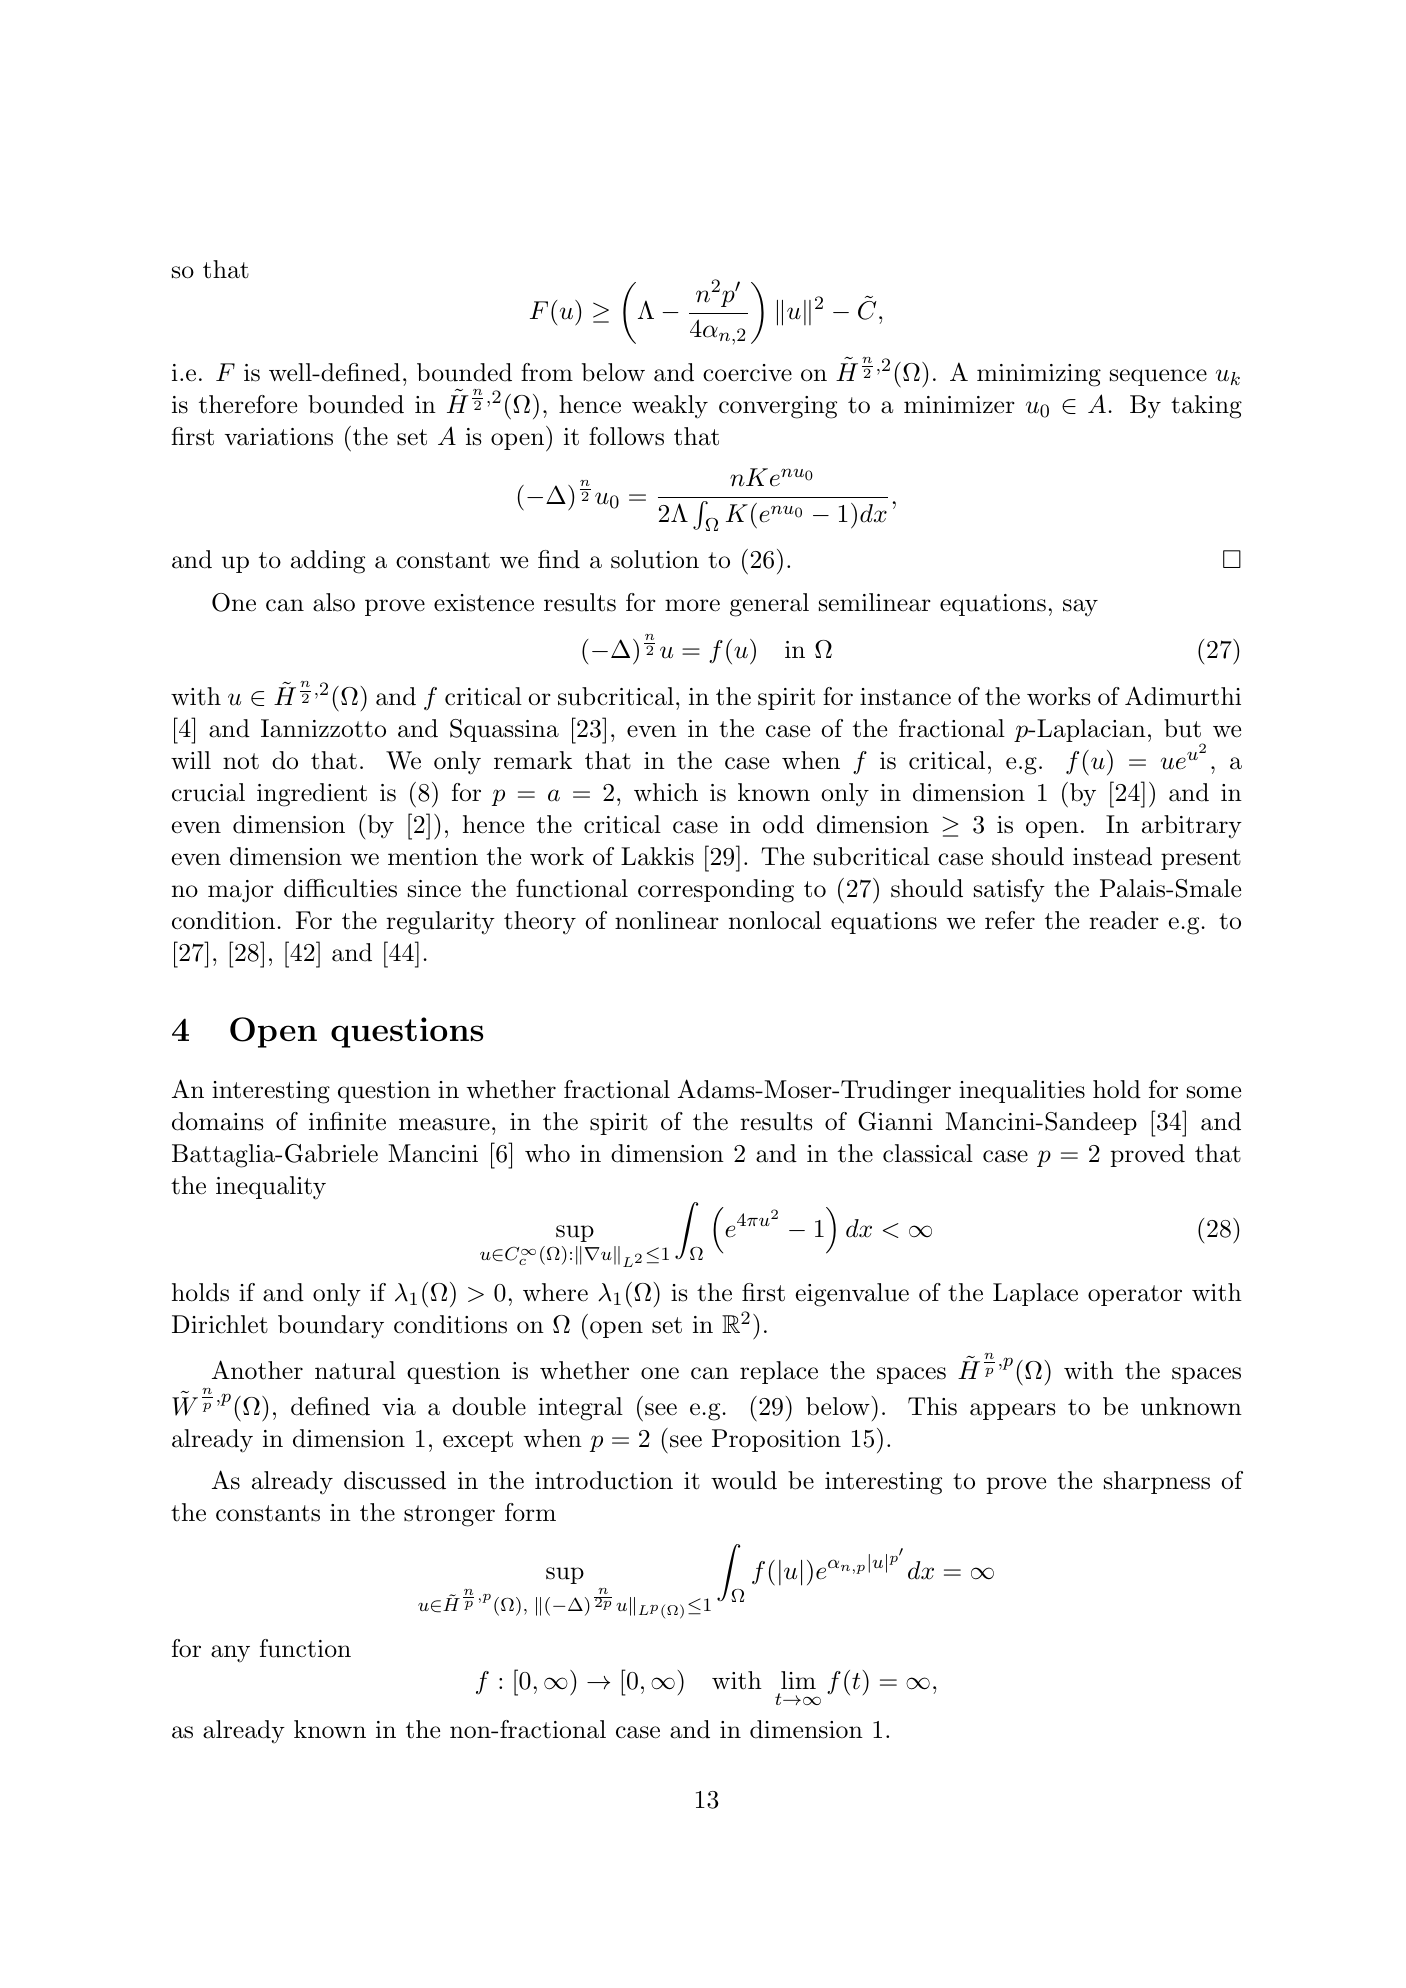
\includegraphics[width=0.96\textwidth,height=0.69\textheight,keepaspectratio]{figures/source_open_questions-13.png}
\caption{Compiled source page 13: the odd-dimensional critical case and all
three questions in Section 4.}
\end{figure}

\section{The theorem-level answer}

Hyder's paper explicitly repeats \eqref{eq:source}, calls it Martinazzi's
question, and proves the following theorem.

\paragraph{Hyder, Theorem 1.1.}
For every finite-measure open $\Omega\subset\R^n$, $1<p<\infty$, and Borel
$f\ge0$ with $f(t)\to\infty$,
\begin{equation}\label{eq:hyder}
 \sup_{\substack{u\in\Htilde^{n/p,p}(\Omega)\\
 \|u\|_{L^p(\Omega)}^p+
 \|(-\Delta)^{n/(2p)}u\|_{L^p(\R^n)}^p\le1}}
 \int_\Omega f(|u|)e^{\alpha_{n,p}|u|^{p'}}\,dx=\infty.
\end{equation}
This is stronger than the requested statement.  Every function admissible in
\eqref{eq:hyder} satisfies
$\|(-\Delta)^{n/(2p)}u\|_{L^p(\Omega)}\le1$, so its admissible set is contained
in that of \eqref{eq:source}.  Divergence over the smaller set forces
divergence over the larger one.  The constant is exactly Martinazzi's
$\alpha_{n,p}$ and the quantifier over slowly growing $f$ is unchanged.

Hyder constructs smooth compactly supported fractional Moser functions and
proves the precise estimate
\[
 \|(-\Delta)^{n/(2p)}u_\varepsilon\|_{L^p(\R^n)}
 \le \left(1+\frac{C}{\log(1/\varepsilon)}\right)^{1/p}.
\]
The $O(1/\log)$ error is the missing precision: after normalization it leaves
the critical exponential mass bounded below while
$|u_\varepsilon|\to\infty$ on a shrinking ball, so any factor
$f(|u_\varepsilon|)\to\infty$ forces divergence.

\paragraph{Hyder, Theorem 1.3.}
For every finite-measure open $\Omega\subset\R^n$, every
$0<\lambda<\lambda_1$, and every $b>0$, there is a nontrivial weak solution of
\[
 (-\Delta)^{n/2}u=\lambda u e^{bu^2}\quad\text{in }\Omega,
 \qquad u\in\Htilde^{n/2,2}(\Omega).
\]
The theorem has no parity restriction, hence it contains every odd
$n\ge3$ highlighted by Martinazzi.  It resolves the displayed model critical
nonlinearity, not every conceivable critical $f$.

\section{Crosswalk and residual scope}

\begin{center}
\small
\begin{tabular}{>{\raggedright\arraybackslash}p{0.25\textwidth}
                >{\raggedright\arraybackslash}p{0.26\textwidth}
                >{\raggedright\arraybackslash}p{0.38\textwidth}}
\toprule
Source item & Later theorem & Exact conclusion \\
\midrule
Strong sharpness for every $f(t)\to\infty$ & Hyder 1.1 & Fully answered yes,
even under the full $H^{n/p,p}$ norm. \\
Odd-dimensional $ue^{u^2}$ equation & Hyder 1.3 & Nontrivial weak solution in
all dimensions for $0<\lambda<\lambda_1$, $b>0$. \\
Replace Bessel by Slobodeckij spaces & Parini--Ruf 1.1; Sk 1.1 & Positive
inequalities and a domain criterion exist for $0<s<1$, $sp=n$, but the exact
optimal exponent was still stated unknown in 2021. \\
Infinite-measure domains & Sk 1.1 & For the Slobodeckij/truncated-exponential
form, validity is equivalent to a fractional Poincar\'e inequality.  This does
not by itself settle the literal Bessel-potential, derivative-only version. \\
\bottomrule
\end{tabular}
\end{center}

Thus no new-proof target remains for the two selected claims.  The exact
Slobodeckij sharp constant is a separate viable problem, but it is not silently
promoted to a resolution here.

\section{Verification}

The source statement was checked in the compiled source PDF, page 13.  Hyder's
question identification and Theorem~1.1 were checked on official arXiv PDF
page 3; Theorem~1.3 was checked on page 5.  The implication from the stronger
full-norm admissible class to Martinazzi's class is immediate set inclusion.
The later-status statements were checked against Parini--Ruf
\href{https://arxiv.org/abs/1607.07681}{arXiv:1607.07681} and Sk
\href{https://arxiv.org/abs/2002.11747}{arXiv:2002.11747}, especially Sk's
Theorem~1.1 and its explicit statement that the optimal Slobodeckij constant
remained unknown.

\begin{thebibliography}{9}
\bibitem{Martinazzi} L.~Martinazzi, \emph{Fractional Adams--Moser--Trudinger
type inequalities}, Nonlinear Analysis 127 (2015), 263--278,
\href{https://arxiv.org/abs/1506.00489}{arXiv:1506.00489}.
\bibitem{Hyder} A.~Hyder, \emph{Moser functions and fractional
Moser--Trudinger type inequalities}, Nonlinear Analysis 146 (2016), 185--210,
\href{https://arxiv.org/abs/1510.06662}{arXiv:1510.06662}.
\bibitem{PariniRuf} E.~Parini and B.~Ruf, \emph{On the Moser--Trudinger
inequality in fractional Sobolev--Slobodeckij spaces}, J. Analyse Math. 138
(2019), 281--300, \href{https://arxiv.org/abs/1607.07681}{arXiv:1607.07681}.
\bibitem{Sk} F.~Sk, \emph{Remarks on the fractional Moser--Trudinger
inequality}, J. Anal. Math. 148 (2022), 323--349,
\href{https://arxiv.org/abs/2002.11747}{arXiv:2002.11747}.
\end{thebibliography}
\end{document}
